\documentclass{article}

% Language setting
\usepackage[english]{babel}
\usepackage{listings}
\usepackage{minted}
% Remove this draft watermark for the final version
% \usepackage{draftwatermark}

% Set page size and margins
% Replace `letterpaper' with `a4paper' for UK/EU standard size
\usepackage[letterpaper,top=2cm,bottom=2cm,left=3cm,right=3cm,marginparwidth=1.75cm]{geometry}

% Useful packages
\usepackage{amsmath}
\usepackage{comment}
\usepackage{graphicx}
\usepackage{IEEEtrantools}
\usepackage[hyphens]{url}
\usepackage[colorlinks=true, allcolors=blue]{hyperref}
\usepackage{array} %table
\usepackage{float} 

\title{PeopleEquity}
\author{Topo Labs (PeopleEquity1@gmail.com)}
\date{\today}

\begin{document}
\maketitle

\begin{abstract}

\emph{PeopleEquity} is a groundbreaking implement of production relationship protocol stack where everyone participates, all participation is recorded, and every contribution is rewarded.

\end{abstract}

\section{Introduction}
PeopleEquity is a unique disruptive narrative of value redistribution with a comprehensive project ecosystem and widespread applications. The product matrix includes: 

\begin{itemize}
   \item \emph{EquitySwap}, the decentralized exchange which automatically increases market depth.
   \item \emph{Production Relationship Protocol Stack}, a Web3 application that reshapes value distribution models.
   \item \emph{Decentralized Credit System (DCS)}, realizes credit traffic monetization, supporting multiple types of on-chain businesses. 
\end{itemize}

\begin{table}[]
\begin{tabular}{lllll}
 &  &  &  &  \\
 &  &  &  &  \\
 &  &  &  &  \\
 &  &  &  & 
\end{tabular}
\end{table}

\renewcommand\arraystretch{1.5} %行高为1.5倍
\begin{table}[htbp] %表格位置
      \setlength{\abovecaptionskip}{0cm} % 调整间距
      \setlength{\belowcaptionskip}{0.2cm}
   \centering
   \caption{\label{tab:l2}DATA SETS} 
   \begin{tabular}{p{2.3cm}<{\centering}p{2.3cm}<{\centering}p{2.3cm}<{\centering}} %列宽和居中
      \hline
      Data set& Total images & Faces \\ 
       \hline
      FDDB& 2845 & 5171 \\ 
      WIDER\_FACE& 30000 & 40000 \\  
      ALFW& 25000 & 25993 \\ 
      \hline
   \end{tabular}
   \begin{tabular}{p{2.3cm}<{\centering}p{2.3cm}<{\centering}p{2.3cm}<{\centering}} %列宽和居中
      \hline
      Data set& Total images & Faces \\ 
       \hline
      FDDB& 2845 & 5171 \\ 
      WIDER\_FACE& 30000 & 40000 \\  
      ALFW& 25000 & 25993 \\ 
      \hline
   \end{tabular}
\end{table}


\begin{table}[h!]
  \begin{center}
    \caption{Multirow and -column table.}
    \label{tab:table1}
    \begin{tabular}{l|c|r}
      \textbf{Value 1} & \textbf{Value 2} & \textbf{Value 3}\\
      $\alpha$ & $\beta$ & $\gamma$ \\
      % \hline
      % \multicolumn{2}{c|}{\multirow{2}{*}{1234}} & a\\ % <-- Multicolumn spanning 2 columns, content multirow spanning two rows
      % \multicolumn{2}{c|}{} & b\\ % <-- Multicolumn spanning 2 columns with empty content as placeholder
      % \hline
      3 & 23.113231 & c\\
      4 & 25.113231 & d\\
    \end{tabular}
  \end{center}
\end{table}


% \begin{table*}
% \label{tab:1}       % Give a unique label
% \begin{tabular*}{\tblwidth}{@{} LLLL@{} }
% \toprule
% Col 1 & Col 2 & Col 3 & Col4\\
% \midrule
% 12345 & 12345 & 123 & 12345 \\
% 12345 & 12345 & 123 & 12345 \\
% 12345 & 12345 & 123 & 12345 \\
% 12345 & 12345 & 123 & 12345 \\
% 12345 & 12345 & 123 & 12345 \\
% \bottomrule
% \end{tabular*}
% \end{table*}



Leveraging blockchain technology, \emph{PeopleEquity} takes an innovative approach to resolve the unbalanced relationships among a project’s many participants and contributors. This enables the many participants in the internet era who provide crucial data to earn deserved labor and equity income. Distributing part of the project's market value growth during its development among participants and contributors narrows the wealth gap, promoting global income equality.

\section{Problem-Solving}

\subsection{Centralized Exchanges Dominate the Crypto Industry}

Despite its decentralized vision, the crypto industry is still dominated by centralized exchanges. According to data provided by CoinMarketCap, as of March 2023, the total trading volume of centralized exchanges exceeded \$2.6 trillion. Calculating the 0.1\% transaction fee that many centralized exchanges charge ordinary users, these exchanges earned up to \$2.6 billion in transaction fees, a figure expected to grow rapidly in the future. At one point, based on Coinbase's trading volume, the total market value of centralized exchanges surpassed the overall crypto market value.

New decentralized blockchain projects are overly reliant on centralized exchanges,  partly due to a lack of transaction frequency on public chains. But more importantly, they are disadvantaged by the flawed underlying pricing principles of current decentralized exchanges, which lead to huge bubbles that form when the growth of liquidity pools is insufficient to support large capital transactions, making it hard for projects to grow independently on decentralized exchanges. 

The success of centralized exchanges is due to the convenience of deposits and withdrawals and the advantages of market depth. Although they contribute to industry development, they cause a significant outflow of funds from the crypto industry into the traditional financial market, weakening the crypto industry. Furthermore, centralized exchanges may also manipulate the market. Under these circumstances, decentralized trading is an unstoppable trend for the sustainable upward development of the crypto space.

Solution: Decentralized Trading Platform \emph{EquitySwap}

EquitySwap is an innovative decentralized trading platform that offers a $three$-in-$one$ solution: \emph{Decentralized exchange}, \emph{Order exchange}, \emph{Futures exchange}.

EquitySwap provides projects with market depth compared favorably with centralized exchanges as well as unlimited development space. This frees projects from dependence on centralized exchanges and achieves completely decentralized trading.

Compared with traditional decentralized trading platforms like \emph{Uniswap}, EquitySwap has the following significant advantages: 

\begin{itemize}
   \item \emph{greater trading depth}, Market depth can automatically increase substantially during the trading process, and when the project's market value rises, its trading depth can be tens to hundreds of times higher than \emph{UniSwap}.
   \item \emph{less impermanent loss}, Impermanent loss is significantly reduced, encouraging more people to add liquidity, thereby increasing EquitySwap and the ecosystem chain's TVL, and making them more likely to take the lead in the corresponding track..
   \item \emph{more trading gains}, TODO.
\end{itemize}

EquitySwap is the first to introduce a mechanism where the project party has pricing power, ensuring the project operates without interference. After the project party or the whitelisted parties add liquidity, other users can then add liquidity. 

EquitySwap has a transaction fee of 0.3\%. The fees are secured on chain and deployed as follows: 

\begin{itemize}
   \item 0.15\% is rewarded to the liquidity providers.
   \item 0.10\% is used for PE and dividends.
   \item 0.05\% is used to distribute equity income and labor income.  
\end{itemize}

The fee income is managed under community supervision, 100\% of the profits are controlled by the community (20\% reserve fund, 80\% used for dividends and buybacks), and are disclosed quarterly. Project participants associated with PeopleEquity's wallets can earn associated trading rewards on EquitySwap when conducting swap exchanges, order trades, futures, and other trades. These rewards are permanently bound to the chain with no performance requirements.

EquitySwap will also launch on-chain order trading features and on-chain future leverage to provide trading functions that traders expect from decentralized exchanges.

In addition, PeopleEquity recommends that application-oriented projects set graduated fees according to traditional fund operating rules as incentives, thereby further motivating all parties.


\subsection{The Internet has changed the Consumer/Production relationship}

In the intenet era, we have seen an interesting phenomenon. The companies that build web platforms realize huge profits and huge capital appreciation (stock price) driven by the work essentially donated by the platform users. Think about Facebook, Youtube, Twitter, etc where the users contribute all, or at least, the majority of the content but do not receive the benefits of the profits and capital appreciation of the company. Hence the emergence of the “internet billionaires”, who profit greatly from the production of the users. The internet era has created a new relationship in business. Traditional relationships were clearly defined, there were “consumers” and “producers”. Today, the internet “users” are the consumers but may also be the producers. Even the simple action of visiting a web site can produce revenue in this era. Amazing!

So the mission of \emph{PeopleEquity} is to enable the users to realize the benefits of relationship. We are changing the value distribution system, so that users and producers can receive the market value (equity) they help to create , i.e., they can earn a portion of the capital gains!

\begin{figure}
\centering
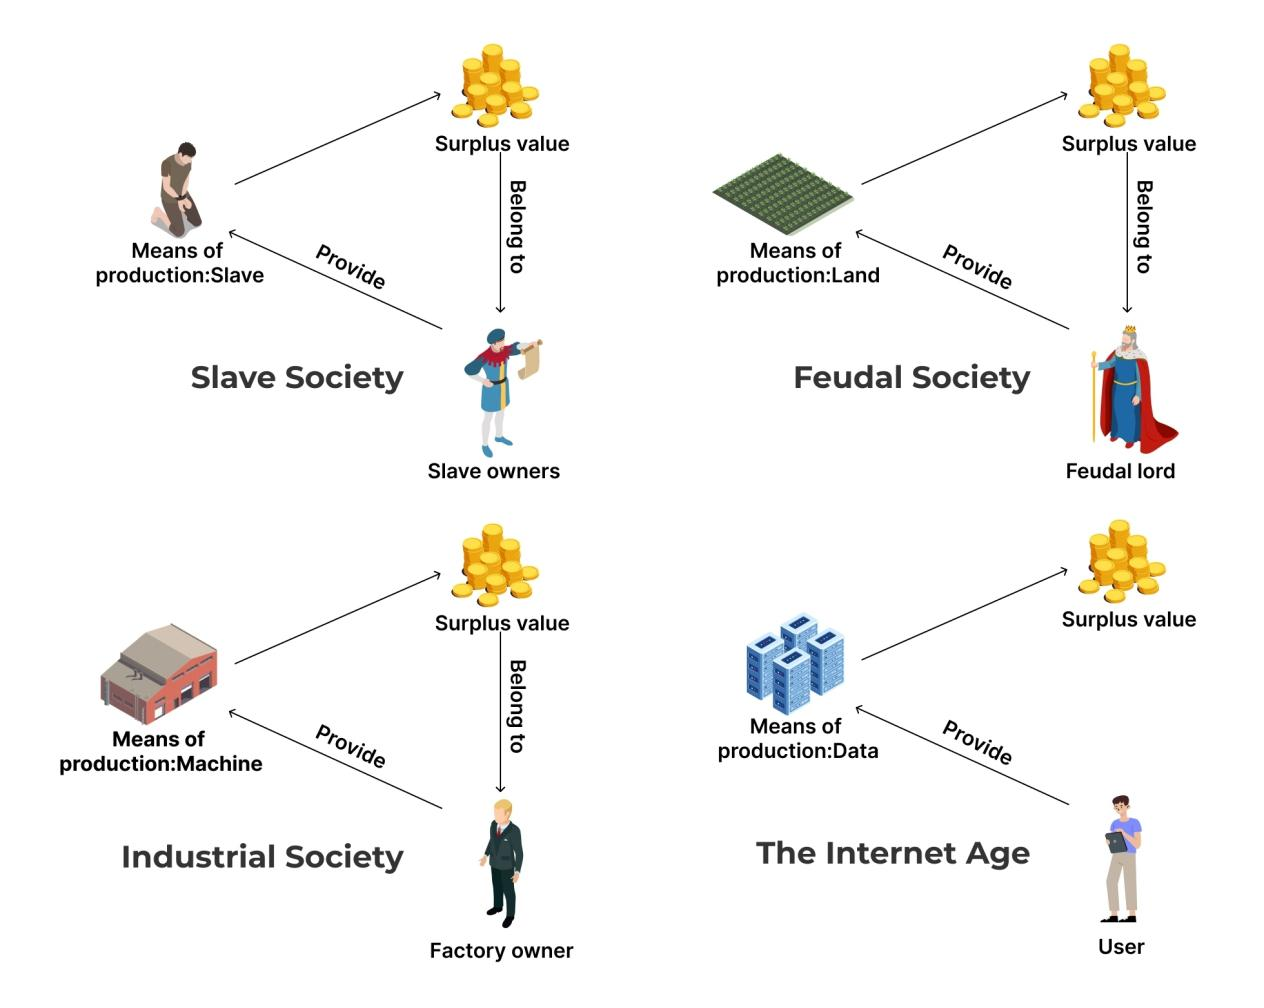
\includegraphics[width=0.6\textwidth]{./img/tranditional_prp.png}
\caption{\label{fig}Traditional Production Relationship Diagram.}
\end{figure}

Solution: Production Relationship Protocol Stack

The \emph{Production Relationship Protocol Stack (PRP Stack)} is the core driver of \emph{PeopleEquity}'s production relationships, composed of several decentralized protocols (VIIP, VSDP, and PEC). The protocol stack is built into PeopleEquity's product ecosystem to address the many challenges and complexities of internet production relationships. 

The \emph{PRP} Stack utilizes blockchain networks to construct a distribution model for each production relationship among the many contributors, including developers, and the many roles of users, so they receive their deserved labor income and equity income via a decentralized system.

Put simply, PeopleEquity eliminates third-parties that could disrupt payments for contibutory efforts, and construct a new business model between users and project applications.

\emph{PE} uses a groundbreaking underlying protocol stack (\emph{VIIP}, \emph{VSDP}, and \emph{PEC}) invented by its innovative R \& D team to define the production relationships and integrate them with the \emph{decentralized credit system (DCS)}. \emph{PeopleEquity}'s decentralized credit system is completely different from other DID solutions; it is a brand new all-scenario credit association network capable of comprehensive association.

Under a defined production relationship, users, as providers of internet production materials, not only gain labor income but may also receive capital-like equity income.


\begin{figure}
\centering
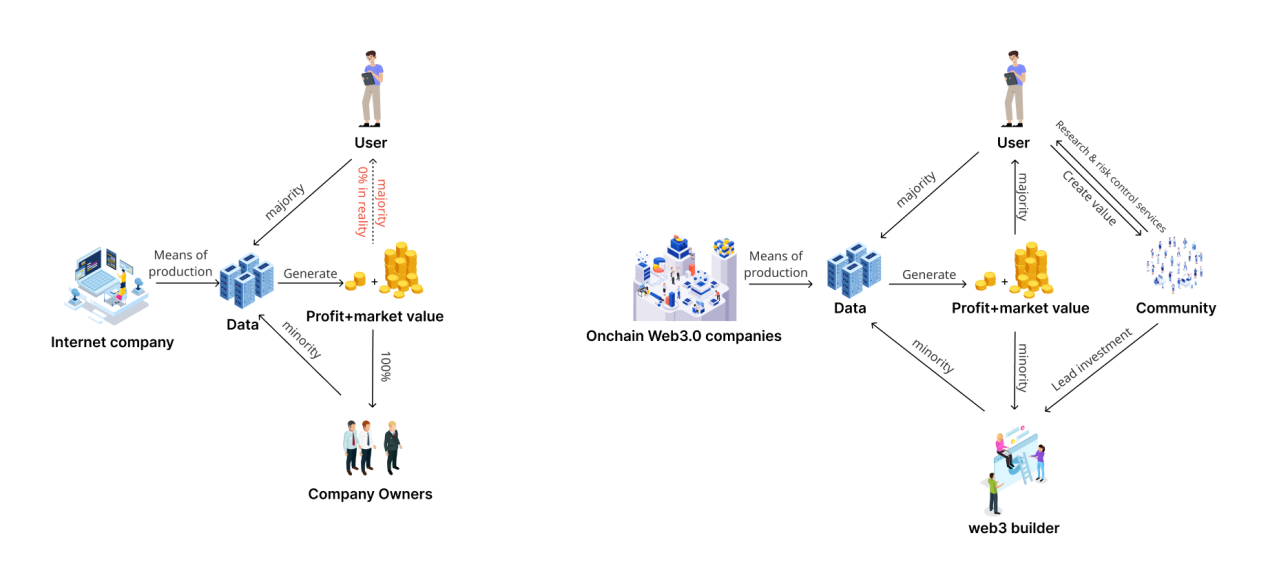
\includegraphics[width=0.9\textwidth]{./img/comparison_prp.png}
\caption{\label{fig}Comparison between Traditional and Web3 Companies.}
\end{figure}


\subsection{Serious Lack of Trust in Crypto}

In crypto, trust is generally lacking. Crypto culture enables outright scam activity and projects with teams that have no intention of creating a lasting project worthy of investment.

These are enabled by a culture that accepts anonymous teams in whom we must place our trust, often blindly. Anonymity is the proverbial two edged sword. It protects our identity and gives us a layer of safety, but it also opens the door to bad actors who can hide and keep their past behavior secret. This is completely contrary to the values and goals of blockchain. 

We urgently need a decentralized credit system that enables the layperson to easily assess the trustworthiness of the people with whom they want to interact. It must be easily accessible, inexpensive, trustworthy, and outside the control of a central organization that could tamper with it. 

The most often spoken phrase in crypto is “do your own research”. A phrase that is easily spoken but near impossible for the common person to actually do when it comes to knowing the credibility of the people we need to trust.

Solution: Decentralized Credit System (DCS)

The PeopleEquity Production Relationship Protocol Stack (PRP Stack) incorporates a Decentralized Credit System (DCS). By incorporating the principles of Decentralized Identity (DID) within the PE platform, users can access information about team players to determine their trustworthiness. The system makes the task of research convenient. DCS revolutionizes the centralized credit system by bringing clear benefits to all parties. Levels of anonymity can be maintained while enabling peer-to-peer queries of on-chain data with open and transparent rules, global coverage, and anti-counterfeiting and anti-cheating functions. (For personal privacy protection, one can choose to reveal their real world identity.)

With the help of the DCS, Decentralized Finance (DeFi) will be able to steadily move towards decentralized credit finance (DCFi). Identities in the DCS are usually anonymous. 

\begin{figure}
\centering
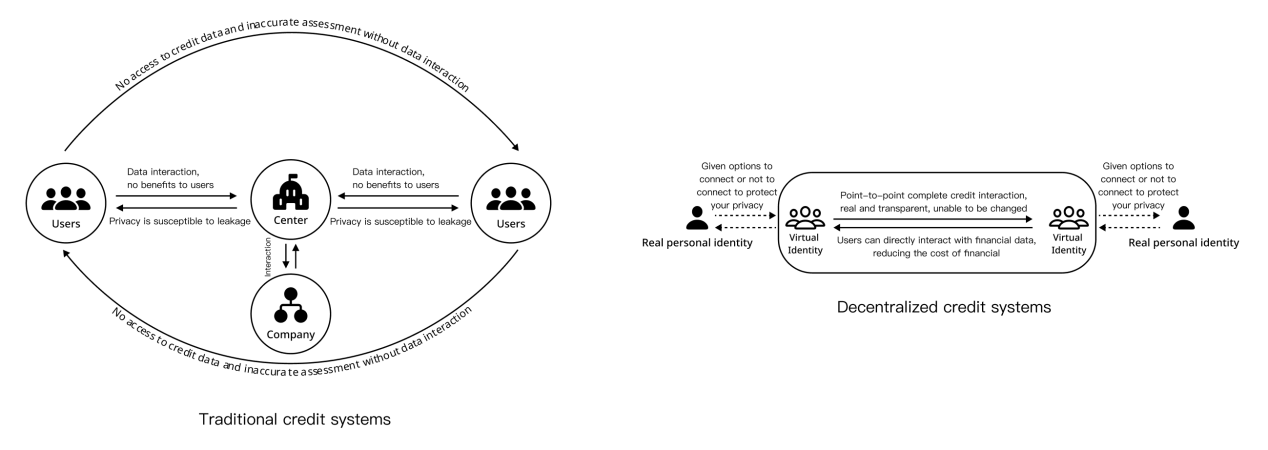
\includegraphics[width=0.9\textwidth]{./img/dcs.png}
\caption{\label{fig}Decentralized Credit System.}
\end{figure}

For those who contribute to a project by participating in social activities the DCS incorporates Proof of Social Activity (POSA) of each virtual identity, which can verify the specific work completed by the user in a certain time. It can also track the social recognition of the work to some extent. 


\section{Theoretical Basis}

\subsection{New Production Relations}
It is fair to state that many internet platform users, especially users of social media platforms realize the inequity of the current systems where contributors are not compensated for the value they contribute to a platforms success. To address this problem, Topo Labs formalizes the consumer-producer relationship, where users receive the labor income and equity income that they produce through their participation. Topo Labs uses blockchain networks to construct the value distribution model, transforming the consumer-producer relationship among developers, contributors, and users in a trustless way without intermediaries like corporations.

The internet consumer-producer relationship has bridged the long-standing gap between users and businesses, achieving a win-win situation through value interconnection. Specifically:

\subsubsection{Users: earn based on contribution}
%\label{subsub:events}

First, users purchasing a companies products are contributing to the company. When a product is purchased, the company not only makes a profit on the item but also gains corresponding securities market income—equity income. For example, user A purchased a product for 500 dollars with a profit of 200 dollars. Calculating the corresponding market value according to a P/E ratio of 40-200, it is about 8,000-40,000 dollars. Assuming the contributed market value is 8,000 dollars, although this 8,000 dollars cannot be fully realized immediately, it is possible to realize 4,000-6,000 dollars by pledging equity. 

Now that user B spends 50,000 dollars to buy a car, the profit of the car is about 15,000 dollars, the P/E ratio of the car company is about 40-200, and the contributed market value (equity income) to the car company is about 600,000-3,000,000 dollars. Obviously, these transactions are not equal, so it is reasonable to distribute the company equity obtained from purchasing services or products to the users according to their contributions.

% Table——Comparison of income and expenditure between users and companies under Web2

In the promotion process of modern Internet companies, sharing is also a very important contribution. Depending on the content of the sharing, it may be physical labor or mental labor. For example, promotional sharing can be classified as physical labor, and the corresponding worker should receive labor income. Sharing with an investment nature requires a lot of analysis and research, belongs to mental labor, and should receive corresponding capital income—equity income. In Web3 companies that use community forms of sharing promotion, it usually involves both physical and mental labor, so such sharing has both labor income and equity income.

% Table——Comparison of income and expenditure between users and companies under Web2

In summary, whether it's user data, consumption activities, or sharing behavior, these are proofs of users participating in the economic activities of enterprises, and are the means of production upon which enterprises rely for profit. The benefits brought to the enterprise should be rewarded accordingly. Under the new production relationship, everyone involved in the project can receive the value of their contributions. Realizing the possibility for everyone to participate, all participation is recorded, and every contribution yields a return.

\subsubsection{Enterprises: Users and Web3 Builders create together}
%\label{subsub:events}

Under the new production relations, users share the dividends of the enterprise, but does this mean that the interests of the enterprise itself are harmed?

First, looking from the consumer market perspective, the additional profits created for enterprises by the new production relations far exceed the loss of equity. As shown in the table below, Web2 users have a staggering wealth gap. Of the existing 4.9 billion internet users, only about 56 million people (net assets greater than 1 million US dollars) have strong purchasing power; 95\% of internet users have extremely weak purchasing power. However, in the Web3 era, new production relations promote income equality. With the efforts of the PE Public Welfare Fund and various sectors of society, people who are not using the internet will quickly join in, and eventually can cover the global population of 8 billion. And due to the reasonable distribution of labor and equity income, equal pay for equal work for user income, these people generally have sufficient consumption power. When the market is infused with fresh blood, the cake will naturally grow larger.


Under the new production relations, local chain supermarkets, and convenience stores, most of the surrounding users own the majority of the equity and dividend rights; tourism accommodation companies, tourists, and individuals providing accommodation own the majority of the equity and dividend rights; logistics companies, logistics delivery staff, and people using logistics own the majority of the equity and dividend rights; for malls, users buying goods own the majority of the equity and dividend rights; for social live broadcast products, social users, and creators own the majority of the equity and dividend rights... In this way, the equity of the enterprise is distributed in a more fair manner to users who contribute to the development of the enterprise, instead of being concentrated in the hands of a few. This will produce a far greater number of rich people and middle-class than the current volume, and their boost to consumption is self-evident.

Secondly, the new production relationship allows enterprises and users to form a community of shared interests. Imagine a new ride-hailing platform, where drivers and passengers complete a business transaction, confirm payment through the blockchain, and can receive equity in the platform. When the majority of the platform's equity and dividend rights belong to users and drivers, the platform will have extremely strong stickiness and growth potential, and ultimately the platform's founders and team will also benefit.

At the same time, compared to the large dilution of Web2 founding team's equity, the equity of the Web3 founding team will hardly be diluted, and the total wealth that the Web3 startup team can get can still be much higher than the Web2 startup team.

% Table——Comparison between Web2 and Web3 companies’ wealth

\begin{figure}
\centering
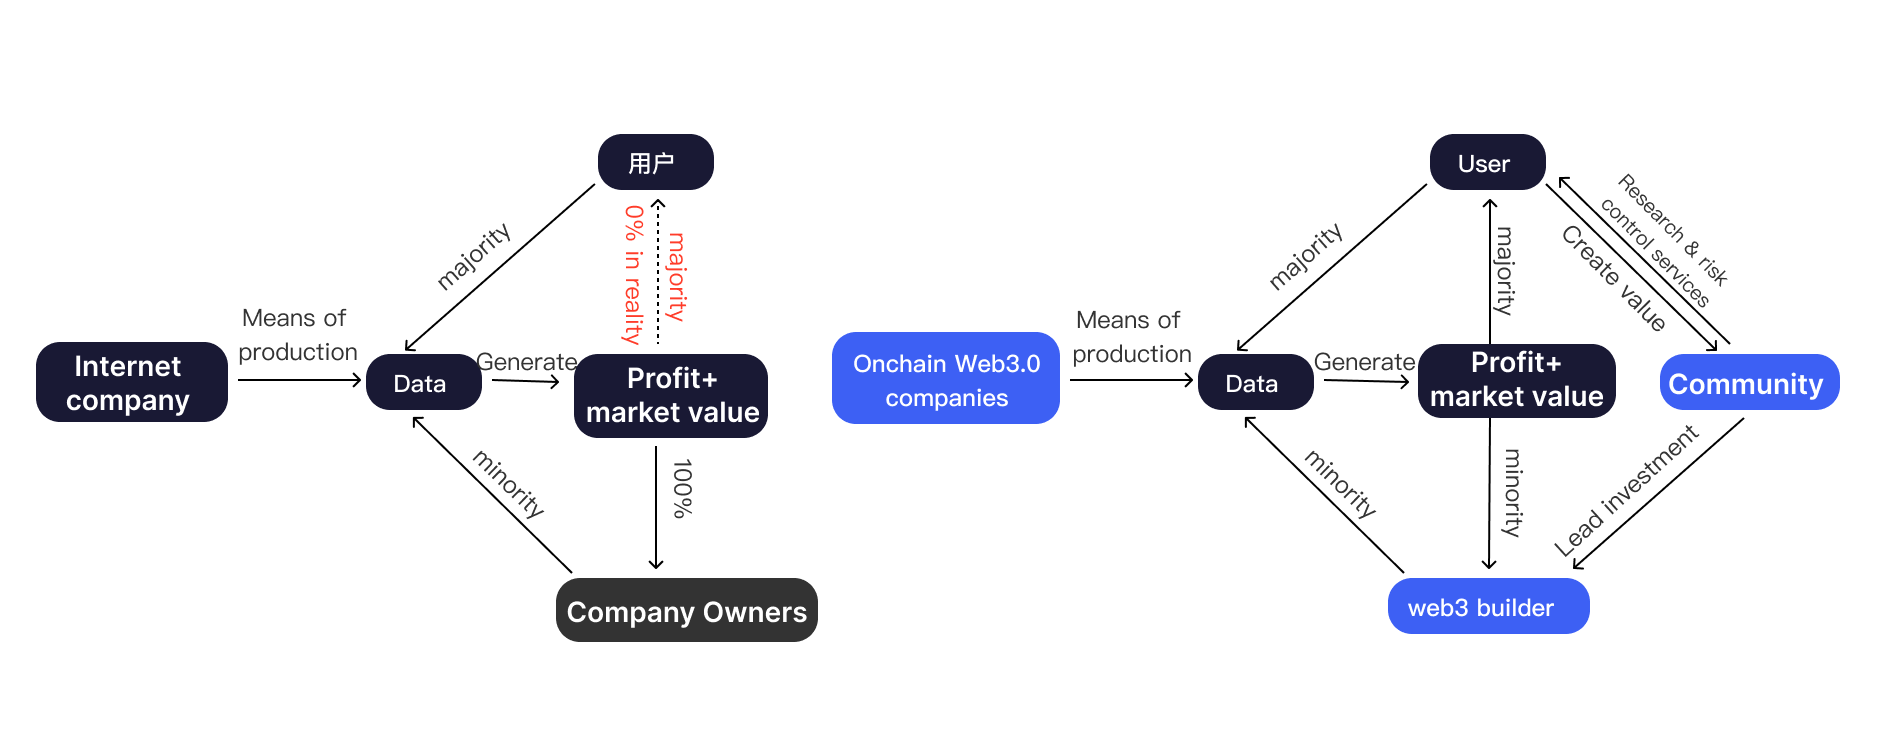
\includegraphics[width=0.9\textwidth]{./img/comparation_production_relation_structure.png}
\caption{\label{fig}New and old production relations structure comparison in the Internet industry.}
\end{figure}

Under the new production relationship, the wealth of the enterprise, especially the equity of the enterprise, is distributed to all participants in a fairer manner. With the significant increase in user wealth, the significant enhancement of consumer confidence and ability, the company's revenue and profits will also grow strongly, which will in turn strongly push the market value of the company and rapidly increase the size of the social cake.


\subsection{New Business Models}

Blockchain technology makes data and value transparent and verifiable, ensuring users' data rights. Although some Web3 projects reward users' "data labor" in various ways, they generally lack solid theoretical support and cannot provide universal solutions. When the user base reaches a certain level and there are no more users to take over, the project ecosystem begins to gradually collapse, narrative logic cannot form a closed loop, and it is difficult to further implement practically. Many projects on the market in Web3 actually do not realize the full benefit of Web3, failing to integrate with real-world business and struggling to gain widespread recognition.

The core members of PeopleEquity have combined interdisciplinary research in history, politics, and philosophy to build the infrastructure for a new business model in the Web3 era, launching universal practical solutions with cutting-edge technology. PeopleEquity believes that Web3 should at least have the following characteristics:


\subsubsection{Web3 should change the current production relations of Web2}

History has proven that unbalanced production relations restrict the development of productive forces and can even lead to widespread social and economic issues. Web3 and blockchain technology have established a decentralized network of trust and value, offering possibilities for transforming production relations. PeopleEquity believes that based on the production relationship protocol stack, a new production relationship suitable for the development of productive forces in the Web3 era can be constructed, reshaping the production relationship and wealth distribution mechanism of Web2.

\subsubsection{Compared to Web2, Web3 should benefit a broader populace}

In modern society, users create profits and securities market value for businesses, and the value of the securities market is often dozens to hundreds of times that of profits. However, as contributors, users only get the use value of goods, which is clearly unfair. Unlike the claims of existing Web3 projects, PeopleEquity believes that users should obtain capital income in addition to ordinary labor income, thus creating a trading environment and wealth distribution model that are fairer. At the same time, PeopleEquity is committed to achieving global income parity, so long as the same labor or cost is expended, the expected return is the same, regardless of the location of the contributor. Nearly 3 billion potential users not yet covered by the internet will join the new ecosystem driven by huge opportunities and benefits. We also set up a fund to help more people who are not using the internet quickly integrate into the Web3 network.

\subsubsection{Web3 should further enlarge market potential to be at least dozens of times larger than Web2}

The size of Web2 is now dozens to hundreds of times that of Web1, and Web3 should achieve a similar multiplication relative to Web2. This expectation is reasonable with the leap in productivity brought about by the new industrial revolution. When society applies new production relations, users will receive their due labor income and equity income, more income will bring corresponding consumption upgrades, further increase corporate profits and market value, and the founding team can also benefit, thus realizing mutual benefits for all parties.

\begin{figure}
\centering
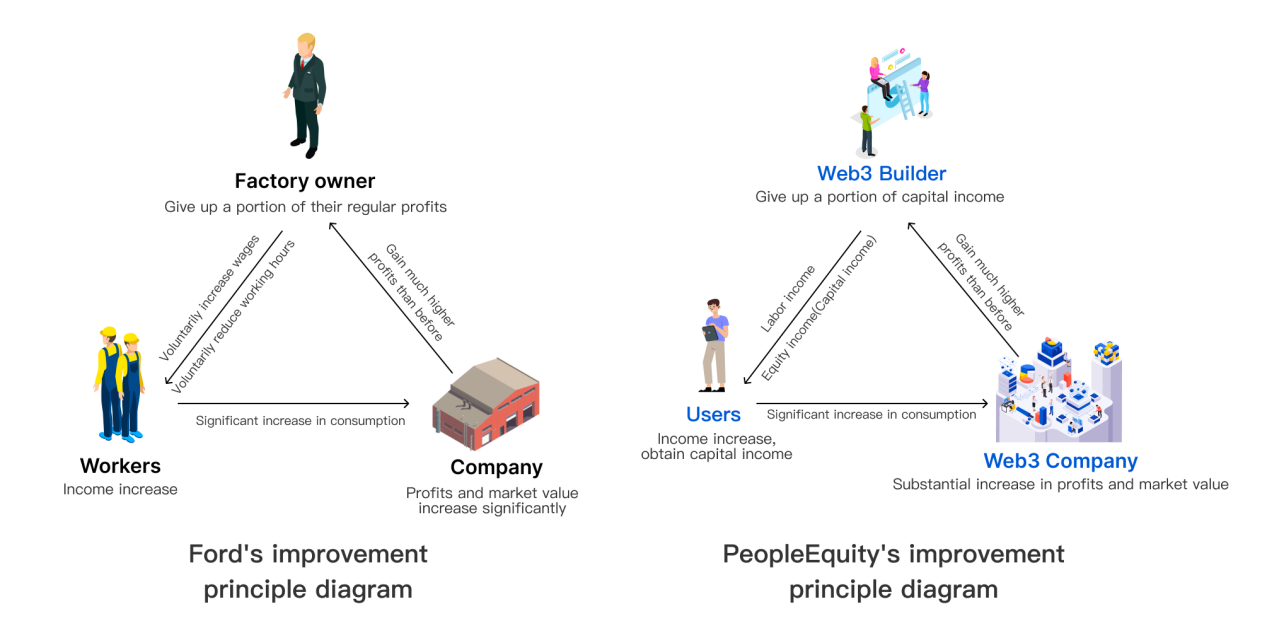
\includegraphics[width=0.9\textwidth]{./img/enlarging_the_cake.png}
\caption{\label{fig}The principle of enlarging the cake to benefit all parties.}
\end{figure}

Data shows that there is an astonishing wealth gap among Web2 users. Among the existing 4.9 billion internet users, there are only about 56 million users with strong purchasing power (net assets greater than 1 million dollars), and the purchasing power of 95\% of internet users is extremely weak. In the Web3 era, new production relationships drive income parity, and with the efforts of the PE public welfare fund and all sectors of society, people who are not using the internet will also quickly enter, and can eventually cover the world's 8 billion population. Due to the reasonable distribution of labor and equity income, and equal pay for equal work, these people will generally have sufficient consumption power. When the market is injected with new participants, the total market value will naturally grow further.

In the new production relationship, local chain supermarkets, convenience stores, and surrounding users own the vast majority of equity and dividend rights; travel accommodation companies, tourists, and individuals providing accommodation own most of the equity and dividend rights; logistics companies, logistics couriers and people using logistics own most of the equity and dividend rights; for shopping malls, users who buy goods own most of the equity and dividend rights; for social live streaming products, social users and creators own most of the equity and dividend rights... In this way, the equity of enterprises is distributed more fairly to users who contribute to the development of enterprises, rather than concentrated in the hands of a few. This will produce a volume of wealthy and middle-class people far exceeding the current volume, the pull on consumption is self-evident.

Secondly, the new production relationship allows enterprises and users to form a community of interests. Imagine a new ride-hailing platform where a driver and passenger complete a business transaction, confirm the payment through the blockchain, and can obtain the platform's equity. When the majority of the platform's equity and dividend rights belong to users and drivers, the platform will have strong stickiness and growth potential, and ultimately the platform's founders and team will also benefit.

\subsubsection{PeopleEquity provides a universal practical solution}

In conclusion, the production relationship protocol stack is a new solution proposed to address the bugs present in internet companies and is also the industry standard for Web3. It can establish Web3 applications suitable for all industries. The decentralized credit system provides credit guarantees for on-chain businesses. EquitySwap provides different listing places for projects of different volumes and provides them with unlimited development space. PeopleEquity is set to open a brand new on-chain business track.


\section{Decentralized Exchange EquitySwap}

\subsection{Technical Highlights}
\subsubsection{Three-in-one Decentralized Exchange}

The three-in-one decentralized exchange offers various listing venues for projects of different initial scales, providing them with unlimited growth space.

\subsubsection{Greater Market Depth}

EquitySwap has improved the underlying pricing principle of a series of previous decentralized exchanges, pioneering an approach that can automatically increase market depth and liquidity pool during the trading process (without manual liquidity addition). When coin prices grow by a higher multiple, the market depth can be tens to hundreds of times higher than Uniswap, and the corresponding capital accommodation capacity and trading capacity will also increase by tens to hundreds of times. This substantial advantage encourages more users to trade on decentralized exchanges, thus allowing funds and traffic to return to the decentralized trading market. It also enables projects to develop independently on decentralized exchanges, reducing reliance on centralized exchanges.

Topo Labs has improved the underlying principles of traditional decentralized exchanges, launching three decentralized exchanges (WhaleSwap, ElephantSwap, and AntSwap) suitable for on-chain businesses of different stages and scales. These exchanges are akin to NASDAQ, the New York Stock Exchange, and the American Stock Exchange, helping on-chain businesses to develop in an efficient and stable way.

\begin{figure}
\centering
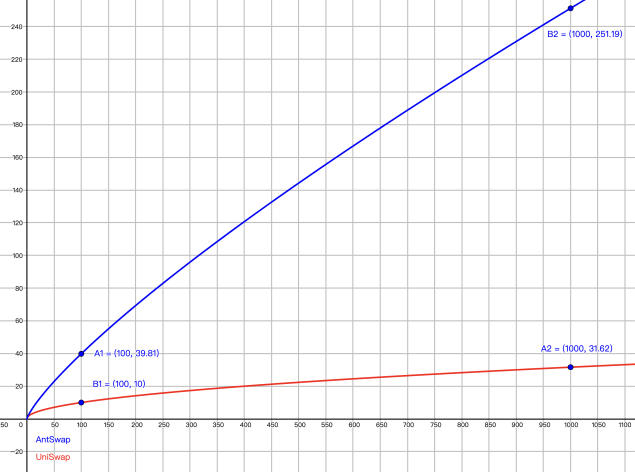
\includegraphics[width=0.45\textwidth]{./img/antswap_uniswap_1.png}
\caption{\label{fig}Comparison of AntSwap and UniSwap liquidity pool with the price growth curve.}
\end{figure}

\begin{figure}
\centering
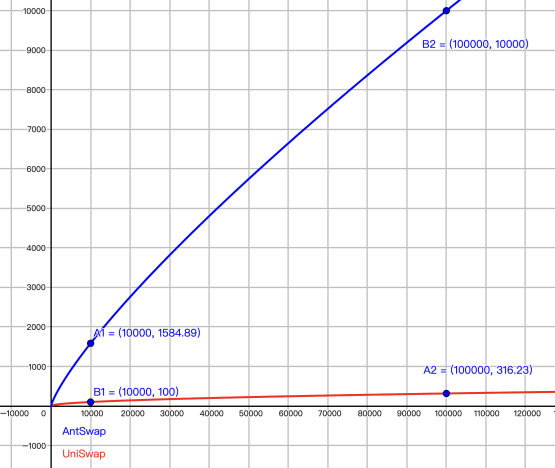
\includegraphics[width=0.45\textwidth]{./img/antswap_uniswap_2.png}
\caption{\label{fig}Comparison of AntSwap and UniSwap liquidity pool with the price growth curve.}
\end{figure}

The above figure assumes that all liquidity pools are in USDT. The horizontal axis represents the multiple of price growth, and the vertical axis represents the multiple of USDT growth in the liquidity pool after the price grows by a certain multiple. As the liquidity pool increases, the accommodatable funds increase, and the number of participants will also increase. Thus, when the project grows by a certain multiple, the market depth can be tens to hundreds of times higher than UniSwap.

\subsubsection{Smaller Impermanent Loss}

EquitySwap's impermanent loss is far less than Uniswap’s, which means more people are willing to add liquidity. Therefore, EquitySwap and its public chain will find it easier to achieve a higher Total Value Locked (TVL). With the same amount of USDT in the liquidity pool, and the same cost for adding liquidity to EquitySwap and UniSwap, after the coin price rises by a high multiple, the remaining value of the former can be tens to hundreds of times higher than the latter.

The below figure compares the impermanent loss curves of AntSwap and UniSwap, showing that AntSwap's impermanent loss is much smaller than UniSwap's.

\begin{figure}
\centering
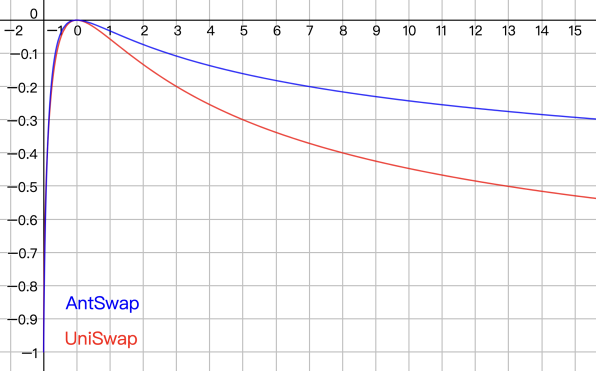
\includegraphics[width=0.45\textwidth]{./img/impermanent_loss_curves_1.png}
\caption{\label{fig}Comparison of AntSwap and UniSwap impermanent loss curves.}
\end{figure}
\begin{figure}
\centering
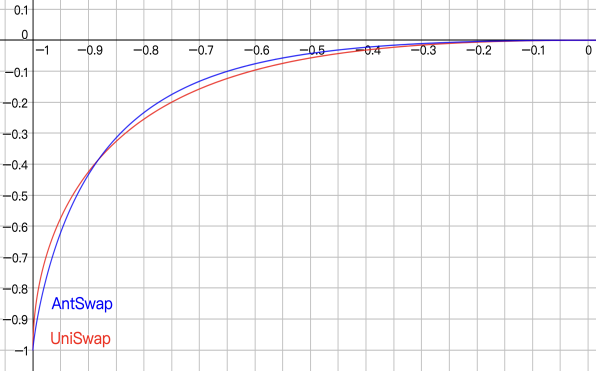
\includegraphics[width=0.45\textwidth]{./img/impermanent_loss_curves_2.png}
\caption{\label{fig}Comparison of AntSwap and UniSwap impermanent loss curves.}
\end{figure}


With the same amount of initial liquidity, when the price increases by a certain multiple, the ratio of remaining funds in AntSwap and UniSwap is as shown in the figure below. The horizontal axis represents the ratio of remaining funds in AntSwap and UniSwap, and the vertical axis represents the multiple of price growth.

\begin{figure}
\centering
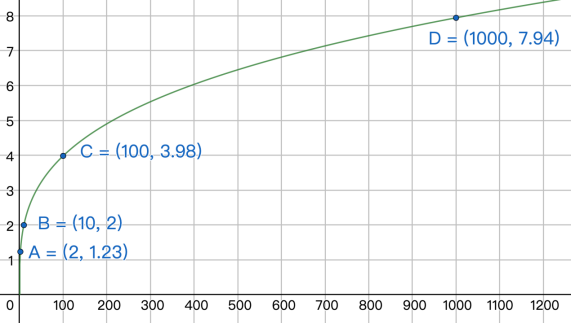
\includegraphics[width=0.45\textwidth]{./img/remaining_funds_1.png}
\caption{\label{fig}Comparison of the ratio of remaining funds in AntSwap and UniSwap.}
\end{figure}
\begin{figure}
\centering
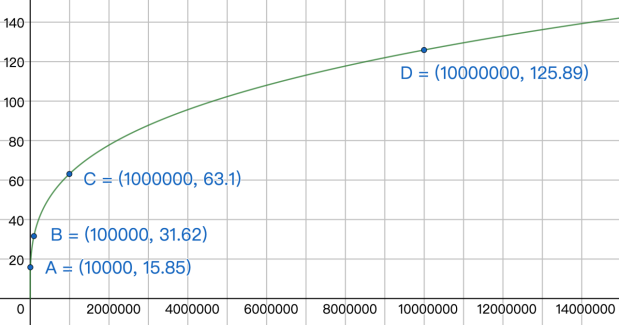
\includegraphics[width=0.45\textwidth]{./img/remaining_funds_2.png}
\caption{\label{fig}Comparison of the ratio of remaining funds in AntSwap and UniSwap.}
\end{figure}


After growing by a high multiple, the remaining funds in AntSwap are tens to hundreds of times higher than the remaining funds in UniSwap. Therefore, more people will be willing to add liquidity to AntSwap.

\subsubsection{Higher Trading Returns (Buy More, Sell More)}

With the same initial liquidity pool in USDT, the same unit price, and the same market value, the same amount of USDT can buy more coins in EquitySwap, and the same amount of coins can sell more USDT, which is a manifestation of greater market depth. In the course of development, when the coin price grows to a certain multiple, the trading returns are also higher at the same price. Simply put, it is "buy more, sell more."

As shown in the table below, when the liquidity pool is the same at 10,000,000 USDT, and the unit price is the same at 1 USDT/token, whether it is the initial market value state (Table 1) or the market value grows to 1,000 times (Table 2) when buying 1,000,000 USDT from the three exchanges, the tokens obtained in the comparison shows that compared with WhaleSwap, which uses the Uniswap traditional exchange pricing formula, trading in EquitySwap's innovative ElephantSwap and AntSwap can exchange more tokens. And when selling 1,000,000 tokens from the three exchanges, ElephantSwap and AntSwap exchange more USDT.


% Table——Effect of Trading Pair Price and Price Fluctuations (Initial Market Value)


% Table——Effect of Trading Pair Price and Price Fluctuations (Market Value Grows to 1,000 times)

\subsubsection{Better Incentive Dividends}

\begin{itemize}

\item Better user income configuration

Compared with UniSwap and Binance, EquitySwap has a clear incentive mechanism, which distributes to users according to their actual contributions by the built-in production relationship protocol stack. Similar to Binance's captain's income, users get labor income and equity income in the process of sharing or promoting. These additional incomes come from the following two parts:

\begin{itemize}
  \item From the income of EquitySwap, this part of the income ratio is the same as Binance, but the growth and expected value are hundreds to tens of thousands of times higher than Binance.
  \item Internal project incentives, the ratio is several times to hundreds of times higher than Binance, and the growth and expected value are still hundreds to tens of thousands of times higher than Binance.
\end{itemize}

The production relationship protocol stack allows users to have equity income when purchasing or using products and services, and users can obtain the market value of their contributions when purchasing or using products, and automatically distribute equity income according to contributions recorded on the chain.

The following table shows the specific shares of labor and equity income:

% Table——ELabor and Equity Income in Investment Trading

% Table——Labor and Equity Income in Product Tsrading

\item More reasonable profit sharing

EquitySwap pioneered the mechanism of project parties having pricing rights to ensure that the project operates normally without interference. After the project party or whitelist adds liquidity, others can add liquidity.

Under community supervision, 100\% of EquitySwap's profits are controlled by the community (20\% reserve fund, 80\% for dividends and repurchases). This mechanism will further enhance the use value of the product, making users true partners in the product.

\item Greater motivation to participate in promotion

EquitySwap makes it more beneficial for users to promote, with a lower threshold for participation. Driven by the above incentives and dividends, users and enterprises form a community of interests, with stronger motivation to participate and promote. The marketing costs saved by the enterprise can be used for truly important technological innovation, with broader development prospects.

\end{itemize}

\subsection{Application Advantages}
\subsubsection{Broader Market}

PeopleEquity provides theoretical support for the implementation of Web3. The production relationship protocol stack enables Web3 to land, while DCS provides credit guarantees for Web3 and significantly reduces commercial and financial costs. As EquitySwap automatically adapts to projects of different initial scales and sizes, it provides a stable development market and unlimited development space for them. The future ecosystem of PeopleEquity will incubate many Web3 application-oriented enterprises. As these companies grow, the scale of Web3 will be two orders of magnitude larger than the current cryptocurrency market.

\subsubsection{Decentralization of Transactions is the Future Trend}

The 3 part decentralized exchange of EquitySwap provides unlimited development space for projects of various initial scales. With the decentralized order book exchange and decentralized futures exchange, the market depth can be comparable to or even exceed centralized exchanges. In a decentralized environment, companies can independently list on decentralized exchanges, avoid market manipulation by centralized exchanges, and avoid "deliberate pinning" scenarios. Decentralization is undoubtedly the trend of the future. EquitySwap provides complete decentralization of Web3 transactions with industry-leading mechanism innovation. It avoids a series of disadvantages of centralization, and promotes the growth of the crypto economy.

\subsubsection{Opening Up a New Web3 Track}

Undoubtedly, Binance currently occupies an absolute leading position in the blockchain ecosystem. However, as the Web3 business continues to develop, it is estimated that its scale will be hundreds of times larger than it is now, which is a huge opportunity. As a leader in the Web3 business track and a hub for the PeopleEquity product ecosystem, EquitySwap has better compatibility than similar products, can better integrate past business tracks, create new decentralized business models, and thereby create greater commercial value.


\section{Production Relationship Protocol Stack}
\subsection{Technical Highlights}
    
PeopleEquity has proposed a new production relationship: users obtain their deserved labor income and equity income. The new production relationship solves the problems that exist in the current Internet companies in terms of production relationships, allowing enterprises, Web3 Builders, and users to form a community of interests, further expand the total market potential, raise the upper limit of social development, and benefit all parties.

Topo Labs analyzed the current corporate structure and built a complete distribution system based on contributiions. Thus, we have implemented the following to enable the Web3 consumer-production relationship.

\begin{itemize}
  \item \emph{Virtual Identity Interconnection Protocol (VIIP)} allows users to establish a credit association network with a clear traceability path around a specific company.
  \item \emph{Value Smart Distribution Protocol (VSDP)} distributes labor income and equity income based on the credit association network. Its topology diagram is an extended star topology.
  \item \emph{Product Equity Certificate (PEC)} applicable to products, recording information related to the transaction parties, including the transacting party, sharing party, and transacted party (or possibly the shared party). The contributions of all parties to the growth of the company will be correspondingly recorded on the chain, and the company will distribute labor income and equity income to all parties based on substantial contributions. Its topology diagram is a network topology. 
\end{itemize}

\emph{VIIP} and \emph{VSDP} are applicable to investments. 

\emph{PeopleEquity} introduces \emph{NFT} as a certificate in both investments and products, as it embodies artistic value and historical value and can fully serve as a digital artwork with both collection and inheritance functions.

In addition, since the production relationship protocol stack belongs to the bottom protocol stack, it is universally applicable to all projects of all public chains, better supporting the landing of the new production relationship in the industry ecosystem.

The diagram of \emph{VIIP} and \emph{VSDP} is as follows:

\begin{figure}
\centering
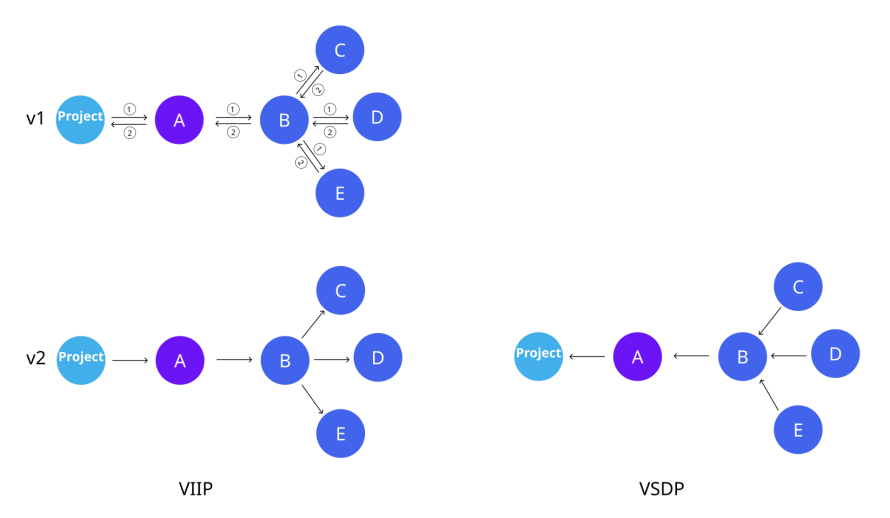
\includegraphics[width=0.5\textwidth]{./img/viip_vsdp_diagram.png}
\caption{\label{fig}VIIP and VSDP Diagram.}
\end{figure}

VIIP establishes a related network, and VSDP distributes corresponding labor income and equity income based on the related network, achieving value-oriented distribution and forming a value internet. It can be applied to various fields, such as production and life. The relevant data on the value of Internet can also provide services for various industries.

\subsection{Application Advantages}

The production relationship protocol stack is the core driver of the new production relationship proposed by \emph{PeopleEquity}, consisting of multiple decentralized protocols (\emph{VIIP}, \emph{VSDP}, and \emph{PEC}). The protocol stack is built into the full product matrix of \emph{PeopleEquity} and the entire industry ecosystem, solving the major bug in the production relationship of the Internet, and using blockchain networks to reshape the value distribution model, transforming the production relationship of the Internet, developers, and users, allowing users to get their rightful labor income and equity income.

From a tangible perspective, \emph{PeopleEquity} is trying to eliminate third-party intermediaries, mainly internet giants, match producers and consumers directly, and build a new business model between users and applications.

In the new production relationship, users as providers of production materials for the Internet, not only get labor income but also further get capital-type equity income.

Comparison Diagram of Traditional Enterprises and Web3 Enterprises
\begin{figure}
\centering
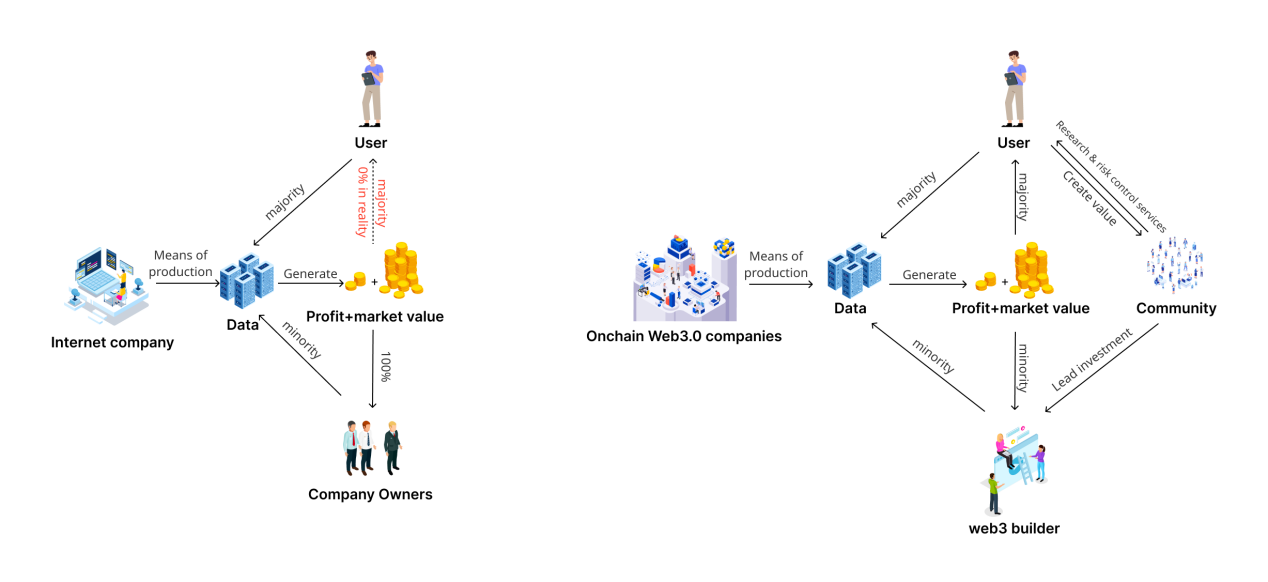
\includegraphics[width=0.9\textwidth]{./img/comparion_web2_web3_company.png}
\caption{\label{fig}Comparison Diagram of Traditional Enterprises and Web3 Enterprises.}
\end{figure}

\section{Decentralized Credit System}
\subsection{Technical Highlights}
The data of the decentralized credit system comes from the internet with a clear traceability path established by VIIP, VSDP, and PEC. PeopleEquity's decentralized credit system is completely different from other DID solutions. It is a new credit correlation network that will reward contributors for the work they do on social media that benefits a project. 

The decentralized digital identity social system correlates contributors’ social activity that is beneficial to the project, reflecting credit through historical data. The system categorizes social activities that users have participated in and records the categorized data in the big data center, ultimately presenting it on the big data platform according to certain rules.

Technically, the decentralized credit system is a sum of Proof of Social Activity (POSA) for each virtual identity individual. POSA can verify the specific work completed in a certain past period and to some extent reflect the social recognition of the work. Specifically, POSA maps the community's comprehensive financial income capability on-chain to the computing power of the blockchain, participates in block production, creates value for the ecosystem, and obtains continuous income.

The decentralized credit system can also be seen as an anonymous digital identity social system based on a smart wallet address, which features anonymity, security, and stability. It can realize point-to-point queries of on-chain credit data, with transparent and public rules, and global coverage. In terms of security, it can prevent forgery and cheating, resist attacks, anti-fraud, anti-censorship, and self-maintenance. In the decentralized credit system, participating parties can achieve mutual success and checks and balances.

\subsection{Application Advantages}

The decentralized credit system, based on the new production relationship proposed by PeopleEquity, injects rules into blockchain commerce. According to open, transparent, and tamper-proof credit data, each investor can view the projects that each project party has developed in the past, and combine other information to judge the growth of the project, thereby reducing the occurrence of blockchain fraud events, purifying the blockchain environment, solving existing industry chaos, fully protecting individual, community, and enterprise interests, and greatly reducing commercial and financial costs.

On the other hand, decentralized credit as the proof of value for social activities and commercial behaviors is also an objective display of personal, community, and institutional investment research capabilities, past achievements, and credit index. It can bring them traffic, directly link to their interests, and promote the continuous realization of credit traffic. Under this credit-based incentive mechanism, establishing and maintaining their own credit will become a spontaneous behavior of entities on the chain, rather than relying on the supervision of authorities and intermediaries.



\subsection{Decentralized Credit Finance (DCFi)}

The decentralized credit system, as the foundation of Web3 and future finance and commerce, will bring a new financial and commercial system to empower commerce and promote industry development.

DeFi is a great financial innovation, it lowers the financial threshold, allowing everyone to directly participate in financial transactions. But DeFi projects, due to the pricing mechanism defects of decentralized exchanges, easily lead to token market value bubbles, liquidity cannot support market value growth, it is difficult to grow independently in decentralized exchanges, must rely on centralized exchanges, so there are very few mass applications; at the same time, DeFi projects have few positive incentive mechanisms, leading to rampant Ponzi schemes, frequent project scams.

PeopleEquity proposed Decentralized Credit Finance (DCFi), which improved the underlying pricing principle of decentralized exchanges, proposed a new production relationship, DeFi will run under the decentralized credit system, empower the real economy, and assist the landing of enterprises' Web3 businesses.

We have difficulty in forcibly punishing individuals who commit fraud on the blockchain, but under the decentralized credit system, individuals and enterprises who commit fraud will have poor credit on the chain and cannot continue.

In DCFi, enterprises and communities play an important role. As companies recognized for entrepreneurship, they should strictly follow the spirit of the contract, sign contracts on the chain with users and investors, and share the profits and market value of the company. With the community responsible for team screening and supervision, as well as the efforts of the teams responsible for maintaining the ecology, enterprises, communities, promoters (KOL \& Influencers), and users form a mutually supervisory, mutually successful community of interest, promoting a virtuous cycle.

Under the guidance of DCFi, all parties work together to participate in the construction of related application projects. The social wealth brought by the application of this process is far greater than the cost of everyone's investment. As total profits are greater than total losses, social wealth continues to increase, realizing a positive cycle.

\subsection{Other Applications}

Visualized credit data can optimize the governance of Decentralized Autonomous Organizations (DAOs), comprehensively contribute data from holding coins and public rules, give members voting rights and decision-making power from multiple dimensions, and let credit become a right to speak. In addition, with the blessing of decentralized credit, NFT, Metaverse, and various Dapps will be re-empowered, stimulating greater financial and social value.

\section{Team Members}

\emph{Topo Labs} is a multinational elite team composed of numerous experts in the blockchain industry and veterans of the crypto industry. Members graduated from world-renowned universities and possess broad theoretical education, exceptional technical strength, and innovative operational capabilities. \emph{PeopleEquity} was created by Topo Labs, which was established to overcome the major theoretical and technical difficulties of the project. Led by the founder and selected team elites, \emph{Topo Labs} is the key driving force behind \emph{PeopleEquity} leading the new Web3 track.

Currently, the team has 15 members and is open to talent globally.

\section{Future Planning}

While realizing decentralized transactions, PeopleEquity will open up a new decentralized business track. We provide a basic protocol stack of production relationships and a decentralized credit system that can reduce business and financial costs for Web3. EquitySwap will be deployed on various popular public chains, and the decentralized credit system will also be established on each public chain.

\subsection{Eco-Development Planning}

\begin{itemize}
   \item First Deployment on BSC Chain and ARB Test Chain.

   EquitySwap and the DCS will be first deployed on the BSC and ARB chains. Collaborating with communities and project teams, we will gradually test the features and enhance EquitySwap's reputation through publicity.

   \item Hosting Various Activities.

   We will host multiple hackathons, providing various types of open-source business contracts to help global entrepreneurs establish blockchain businesses in various industries.

   \item Testnet Launch + Mainnet Launch.

   The ESChain testnet will be open for public testing in late May 2023. In August 2023, ESChain's mainnet will go live, EquitySwap will be deployed synchronously to the ESChain mainnet, and MyShop, the first blockchain-based physical shopping mall project, will be launched on ESChain's mainnet and listed for liquidity trading on EquitySwap.

   \item Rolling Out Other Business Ecosystems.

   We will successively launch blockchain-based tourism accommodation, lifestyle peripherals, and transportation projects.

   \item Fully Open-source Commercial Projects to Further Promote Industry Development.

   The source code of MyShop will be fully open-source within two months of its launch, followed by other projects on the chain.

   \item Tackling Dynamic Sharding.

   ESChain will tackle dynamic sharding within 6-8 months, achieving a real TPS of 1 million+ to accommodate the explosive growth of on-chain commerce. 
\end{itemize}

\subsection{Publicity Planning}

\begin{itemize}
   \item Media.

   We will promote our philosophy on blockchain vertical media, traditional media, and various communities, and Web3 platforms. We will release related introduction videos on major video platforms to increase project awareness.

   \item Test Activities.

   When we have a sufficient user base, we will attract loyal users from the blockchain and Web2 through multiple rounds of testing on the protocol stack of production relations, a decentralized credit system, and a decentralized exchange.

   \item Hackathons.

   We will host multiple hackathons and startup competitions to expand the on-chain application.

   \item Support Plan.
   
   We will set up a support plan, solicit project entries, provide resources from the PeopleEquity ecosystem for the projects, and support their development with funds and technology.

   \item Conclusion and Outlook.

   The new production relations led by PeopleEquity, based on the decentralized credit system, centered on the contribution of participants, and distributing labor and equity income, will ultimately achieve a fairer wealth distribution. Under this new production relationship, as enterprises and users form a community of shared interests, users share the dividends of enterprise development, and enterprises create better economic benefits. PeopleEquity and the new production relations model will lead economic and social development into the future, and the wealth of society will continue to grow.
\end{itemize}

% Reference style
\bibliographystyle{IEEEtran}
\small{
    \bibliography{bibtex}
}
\end{document}